%! TEX root = ../main.tex
\section{Educación Tradicional}

La educación tradicional o instruccionismo se basa en la transferencia de 
conocimiento del profesor al alumno, se enfoca más en el profesor, en la 
capacidad del mismo, y en el producto final como resultado de un proceso 
no interactivo y bien documentado\cite{igi:instructionism}. Los mecanismos 
tradicionales para probar la efectividad de este tipo de enseñanza son los exámenes.

%\fixme{La educación tradicional o instruccionismo se basa en el concepto de que
%   existe un profesor y un alumno. El profesor transfiere el conocimiento que
%    ha adquirido de diferentes métodos (educación, experiencia, etc) a un alumno
%    que es un receptor pasivo de información }{No copy/paste en la
%    intro}\cite{johnson2005instructionism}.

%Se enfoca más en el profesor, y en la enseñanza, y en el producto final como
%resultado de un proceso no interactivo y bien
%documentado\cite{igi:instructionism}. Los mecanismos tradicionales para poder
%probar la efectividad de este tipo de enseñanza son los exámenes.

%\fixme{La principal}{Ablandar} critica a este modelo es que se enfoca la
%enseñanza y no el aprendizaje, mientras más se enseña, más se aprende.
%\textbf{Esto contradice al sentido común en el sentido de que, cosas básicas
%    como caminar o hablar, aprendemos sin la necesidad de un
%    profesor\cite{ackoff:education}\cite{johnson2005instructionism}.}{Más
%    énfasis en el aprender haciendo y usar referencias, no ``el sentido común''}

Una de las principales criticas a este modelo de enseñanza por parte de las
demás corrientes pedagógicas es que según ellas el instruccionismo se basa en la
idea de que  \enquote{cuanto mas se enseña mas se aprende} y esto contradice al
enfoque de \enquote{aprender haciendo} teniendo en cuenta que cosas como caminar
o hablar se aprende sin la necesidad de un profesor
\cite{ackoff:education,johnson2005instructionism}. 

%Tradicionalmente el rol de las TIC's en la educación se vio relegada a la de
%sustituto del libro y/o de presentaciones en clase, es decir, es un mecanismo
%más para trasmitir el conocimiento del maestro al alumno.



\section[Educación con TIC's]{Educación con las Tecnologías de la Información y
    Comunicación}
\label{sec:tics_educacion}

Las expectativas iniciales acerca del impacto de las \Gls{tic} en la educación
fueron ampliamente superiores a los resultados obtenidos\cite{unesco:ict}. Con
el advenimiento de las computadoras se redujo esta diferencia entre las
expectativas  y lo obtenido, en mayor medida por que se utilizo a las \Gls{tic}
en conjunto con  tecnologías como Internet, y los efectos positivos en la
educación fueron aumentando gradualmente\cite{unesco:ict}.

Una de las principales ventajas de la utilización de las \Gls{tic} en la
educación es su aplicabilidad en áreas como:

\begin{itemize}

\item \textbf{Nuevos modelos pedagógicos:} teorías como el constructivismo moderno
    enfatizan el proceso de como adquirir (aprendizaje) conocimiento y no
    solamente como transmitir el conocimiento en sí (enseñanza).

\item \textbf{Eliminación de distancias:} Con la aparición de las computadoras y los
    satélites,  el mundo se ha convertido en una aldea global, y las distancias
    en cuestiones de transmisión de información se han vuelto
    insignificantes\cite{mohammed2013information},  los medios tradicionales
    como bibliotecas, o escuelas están limitados a un espacio  físico, con el
    uso de las \Gls{tic}, esta restricción física desaparece\cite{tinio:ict}.

\item \textbf{Colaboración distribuida:} como consecuencia del punto anterior, los
    alumnos pueden colaborar de manera más sencilla pues no tienen limitaciones
    físicas. Además, los alumnos pueden consultar con expertos que están en
    linea, e incluso tener mentores en linea, estas tutorías pueden ser uno a
    uno, por ejemplo mediante comunicaciones por correo electrónico. Además
    permite la colaboración masiva entre estudiantes de intereses comunes,
    mediante foros y redes sociales\cite{unesco:ict}.

\item \textbf{Motivación para aprender:} Las \Gls{tic} tienen un impacto positivo en el
    proceso de aprendizaje especialmente en lo referente al compromiso
    con\cite{passey2004motivational,egenfeldt2007third}:
	    
    \begin{itemize}
    \item La actividad: a través de estímulos visuales, auditivos, etc.
    \item La capacidad de investigación: es más fácil acceder a gran cantidad de
        información bibliográfica.
    \item La capacidad de escritura y lectura: emitiendo compartir  ideas de
        manera más legible y mejorarlas iterativamente.
    \item La capacidad de presentación: es más fácil presentar trabajos
        profesionalmente a un público mayor.
    \end{itemize}
	    
\item \textbf{Adquisición de habilidades básicas:} las habilidades necesarias para
    utilizar de manera efectiva las \Gls{tic} se están convirtiendo en una
    necesidad básica, un aprendizaje guiado por las mismas puede ayudar a una
    rápida asimilación de los conceptos \fixme{relacionados}{Por qué?}.

\end{itemize}

Uno de los desafíos más importantes que enfrentan las \Gls{tic} para convertirse
en una alternativa viable es la inversión en infraestructura
necesaria\cite{unesco:ict}.

\subsection{Evolución}

La historia de las \Gls{tic} en educación comienza en la \enquote{Open
    University of United Kingdom} que en $1969$ se establece como la primera
institución educativa dedicada a la enseñanza a distancia utilizando las, para
aquel entonces, nuevas tecnologías\cite{tinio:ict}. 

El análisis de la historia de las \Gls{tic} en educación es indispensable,
aunque existe una corriente que tiende a desestimar las experiencias pasadas,
cuyo principal fundamente es la velocidad con la que la tecnología evoluciona,
es importante el estudio de la evolución de la misma pues los errores
pedagógicos cometidos, aunque puedan parecer evidentes hoy en día, condujeron a
nuevos modelos y conclusiones que son la base de la utilización de las \Gls{tic}
hoy en día\cite{mcdougall2006theory}.

El impacto de las \Gls{tic} en la educación no ha sido constante durante su
historia, sino más bien, ha evolucionado de ser un medio más de traspaso de
información, hasta hoy en día, donde permite generar
conocimiento\cite{tinio:ict}.

\begin{figure}
    \centering
    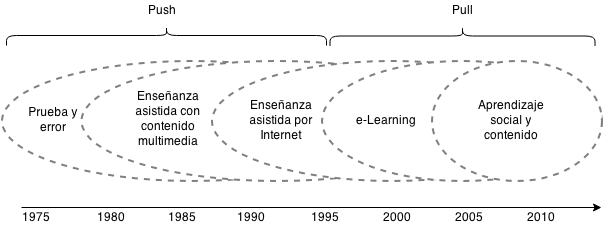
\includegraphics[scale=0.75]{tics/images/tics_history.png}
    \caption{Utilización de las \Gls{tic} en la educación desde el año $1975$}
    \label{fig:history_tics}
\end{figure}

Para entender la historia de las \Gls{tic} en la educación, se presenta el
gráfico~\ref{fig:history_tics}, en el cual se observa la evolución que sufrió la
utilización de las \Gls{tic} como herramienta en la educación. Se observa que se
parte la historia en cinco corrientes definidas, y a la vez, estas corrientes se
agrupan según el mecanismo de obtención de información, las tres primeras
corrientes se denominan \textit{pull} y las siguientes dos se denominan
\textit{push}. \textit{Pull} se refiere a que los estudiantes obtenían la
información sin participar en la creación de la misma, y \textit{push} es cuando
los alumnos son creados activos de conocimiento\cite{white:ict,leinonen:ict}.

Aunque la figura~\ref{fig:history_tics} muestre un progreso lineal de las
corrientes, este progreso no es igual en todo el mundo, y la el grado de impacto
de las \Gls{tic} varia entre países, lo que se conoce como una brecha
tecnológica. Las fechas utilizadas en el figura~\ref{fig:history_tics} son
relacionadas a la evolución en los Estados Unidos de Norte America.

\subsubsection{Pull}

A finales de la década de $1970$ e inicios de la década de $1980$,  la
complejidad técnica de las computadoras limitaba la cantidad de herramientas
disponibles, los programas eran desarrollados por profesores, y su objetivo era
que los alumnos puedan poner en práctica lo aprendido en el aula. El campo de
aplicación de las herramientas se limitaban a matemáticas y lenguaje, donde se
podía evaluar inmediatamente los resultados proveídos por los alumnos, pues,
normalmente era un enunciado y una lista posible de opciones. La cantidad
limitada de opciones para responder, provocó que los alumnos no interpreten los
resultados, sino prueben todas las posibles opciones hasta pasar al siguiente
enunciado, sin realizar ningún aprendizaje significativo\cite{leinonen:ict},
este tipo de juegos se denomina \enquote{Prueba y Error}.

Cuando aparecieron en el mercado computadoras con multimedia, a finales de la
década de $1980$, la utilización de las \Gls{tic} se simplificaron y dieron
contenido a la posibilidad de incluir contenido multimedia, se argumentó que los
ejercicios de tipo \enquote{Prueba y Error} no cumplieron su objetivo de una
educación profunda por que no contenían multimedia\cite{leinonen:ict}, así, en
se empezaron a distribuir las aplicaciones eran distribuidas por
\textit{CD-ROM}, se actualizaban de manera frecuente, y podían contener gran
cantidad de contenido multimedia.

Con la creación de los juegos del tipo \enquote{Prueba y Error} y el contenido
multimedia, se inicio a un nueva corriente denominada \emph{Edutainment},
palabra que representa la unión de la educación y el entretenimiento. Así el
\emph{edutainment} pretende agregar entretenimiento a la educación, se ve al
alumno como un receptor pasivo de información que debe asimilarla, y para
aumentar la implicación de los alumnos, el entretenimiento era
agregado\cite{resnick:2004}.

Los \emph{edutainment} se basan principalmente en el conductismo y el
cognoscitivismo, se enfoca en juegos sencillos que transmiten información simple
al usuario, su estructura se basa en un objetivo claro que está separado de la
experiencia educativa\cite{egenfeldt2007third}. 

\emph{Math Blaster} (ver~\ref{fig:math_blaster}) es un \emph{edutainment} donde
el alumno debe responder repetitivamente preguntas aritméticas para obtener
municiones, luego con esas municiones debe completar diferentes misiones en una
nave\cite{bruckman1999can}. Como todas las preguntas se responden mediante un
mecanismo de selección múltiple, y no existe penalización por fallar una
respuesta, los alumnos no reflexionan sobre las respuestas elegidas, seleccionan
una opción aleatoria y si no es la correcta, prueban otra, tras una cantidad
finita de intentos, siempre se obtiene la recompensa deseada.

\begin{figure}[ht!] 
\centering 
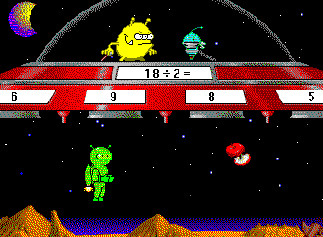
\includegraphics[scale=0.5,natwidth=296,natheight=217]{tics/images/math_blaster.jpg}
\caption{Math Blaster, \emph{edutainment} del año 1987}
\label{fig:math_blaster} 
\end{figure}

\begin{figure}[ht!] 
\centering 
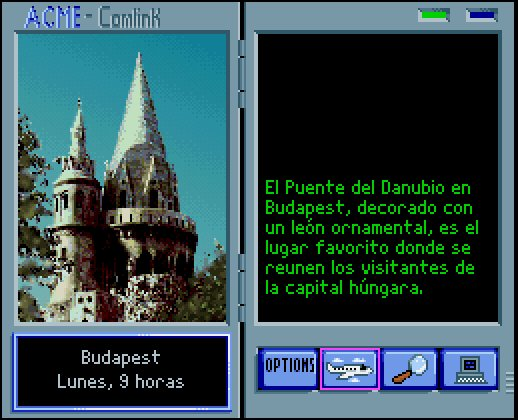
\includegraphics[scale=0.5]{tics/images/carmen.jpg}
\caption{Donde en el mundo esta Carmen Sandiego} 
\label{fig:carmen}
\end{figure}

\enquote{Donde en el mundo esta Carmen Sandiego} (ver~\ref{fig:carmen}) es un
juego que representa el potencial multimedia de esta época, el objetivo del
juego era detener a una serie de criminales mediante una serie de pistas que
eran provistas en forma de texto. Este exitoso juego demuestra las falencias de
esta época, siendo visualmente muy atractivo, y con contenido multimedia acorde
a su tiempo, no era más que \emph{prueba y error}, cada nivel del juego podía
ser completado sin leer la información proveída educativa\cite{charsky:2010}.

Los \emph{edutainment} no logran enseñar habilidades complejas, se enfocan
principalmente en enseñar tareas extremadamente repetitivas que no dependen de
un contexto\cite{charsky:2010,egenfeldt2007third,bruckman1999can}, son
excelentes para enseñar a sumar, pero no para aplicar ese conocimiento, analizar
y obtener conclusiones, o evaluar lo que aprendieron.

Las principales causas por del fracaso de los \emph{edutainment} en su intento
de ser una alternativa viable a la educación son según\cite{egenfeldt2007third}: 

\begin{itemize}

\item \textbf{Falta de motivación interna:} los \emph{edutainment} se centran en
    motivaciones externas, y dejan de lado la motivación interna. Se centran en
    dar recompensas por acciones lo que es una motivación externa, que en que el
    alumno se sienta emocionado al finalizar un nivel, lo que es una forma de
    motivación interna.

\item \textbf{Aprendizaje como anexo:} el principal objetivo del desarrollo de un
    \emph{edutainment} es el de entretener, los objetivos pedagógicos son
    agregados al final. Adicionalmente, este aprendizaje se provee a través de
    largos textos que normalmente son omitidos.

\item \textbf{Interacción limitada:} son construidos con una jugabilidad pobre,
    sin la posibilidad de realizar multiples acciones, normalmente limitados a
    seleccionar respuestas o moverse en un pequeño mundo. 

\item \textbf{Ejercicios de prueba y error sistemáticos:} todas las debilidades
    anteriores se pueden fundamentar en el hecho de que los juegos permiten al
    alumno intentar varias veces sin ser penalizados, además
    de que los alumnos no están motivados, provocaba que todas las opciones sean
    probadas sin el proceso de reflexión necesario para aprender, por ejemplo,
    varios juegos aritméticos solicitaban pruebas del tipo $2+2$ donde el alumno
    probaba diferentes resultados y luego memorizaba el mismo. Se enseñaba a
    probar opciones sin sentido antes que entender y analizar la experiencia.

\end{itemize}

Los \emph{edutainment} se limitan a enseñar tareas mecánicas, sin entender el
contexto en el que se aplican y por qué se realizan\cite{egenfeldt2007third}.

El contenido distribuido, aunque contribuyo a la calidad del contenido proveído,
no resolvió el problema de contenido actualizado, pues a comienzos de la década
de $1990$, con la popularización de Internet\footnote{Internet se concibió lo
    que hoy se conoce como \emph{World Wide Web}\cite{white:ict}, pero se
    masifico en la década de $1990$\cite{leinonen:ict}}, se genera más contenido
que el que puede ser distribuido por medios físicos, así se accede al tercer
hito de la figura~\ref{fig:history_tics}, donde el contenido es distribuido por
internet.

Las bases pedagógicas de los \emph{Edutainment} siguen siendo las mismas, la
incursión de internet solo permite contenido actualizado, los problemas
persisten y se crean nuevos factores que incrementan la brecha tecnológica,
ahora, además de poseer una computadora, es necesaria una conexión permanente.
La velocidad inicial de internet no es suficiente para proveer los mismos
entornos ricos en multimedia que sí lo proveían los CD-ROM\cite{leinonen:ict}.

Así se crea una nueva generación de \emph{edutainment}, que son distribuidos por
internet, actualizados constantemente, pero con los mismos problemas
\cite{leinonen:ict}.

Un cambio de paradigma permite poner fin a la época de los \emph{Pull}, se pone
especial énfasis en el aprendiz y no en el contenido, así se inicia la época
\emph{Push}.

\subsubsection{Push}

Se inicia con el \emph{E-Learning}, \emph{E-Learning} se define como la
educación y capacitación a través de medios digitales, incluye todo tipo de
medio capaz de distribuir información, puede ser de en tiempo real como
salas de conversaciones y videoconferencias o puede ser diferido, como por
ejemplo foros, enciclopedias. Es particularmente útil para educación a distancia
y con horarios flexibles. Se originó a finales de la década de $1990$ y tuvo su
apogeo a mediados de la década del $2000$, apoyada por la gran penetración de
las \Gls{tic} en la población\cite{punie:ict}.

Se distribuye contenido masivamente a los alumnos, y luego, de manera discreta
se permite a los mismos colaborar, dejando siempre en claro que primero se debe
asimilar toda la información posible y luego relacionarse con los
demás\cite{leinonen:ict}, esto evidencia algunos problemas pedagógicos heredados
de la época \emph{Pull}.


\begin{figure}[h] 
\centering 
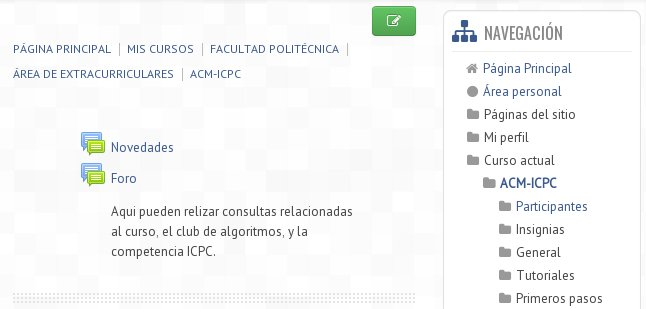
\includegraphics[scale=0.5]{tics/images/moodle.jpg}
\caption{Moodle, plataforma de e Learning} 
\label{fig:moodle}
\end{figure}


La plataforma \emph{Moodle} (ver~\ref{fig:moodle}) cuya primera versión salió en
el $2002$, es una de las principales herramientas del \emph{e-Learning} hoy en
día, permite la creación de cursos específicos por materia y sitios
especializados por instituciones académicas\cite{perkins2006using}. 

La utilización del \emph{e-Learning} tiene varios grados de aplicación en
entornos reales\cite{punie:ict}, que van desde ser simples elementos
complementarios a la clase, como por ejemplo un repositorio para las
diapositivas y otros materiales de clase, hasta cursos completamente en línea,
donde la clase ha sido completamente sustituida.

Sí bien, el \emph{e-Learning} permite la distribución y colaboración en
distintos niveles, no hace un enfoque en el aspecto pedagógico, y se centra en
la forma de transmitir información, y no como la recibe el
alumno\cite{leinonen:ict}.

Ideas que surgieron en la época \emph{Pull} son tomadas en cuenta a la hora de
diseñar nuevos esquemas de educación\cite{mcdougall2006theory}, las teorías del
construccionismo de \textit{Papert}, permiten enfocarse en el alumno, además del
ambiente en el que ocurre el aprendizaje\cite{egenfeldt2007third}.

